\chapter{Aprendizado de regras}

Nas seções seguintes mostraremos resultados da capacidade de autômatos celulares reproduzirem padrões de estruturas secundárias a partir da sequência de aminoácidos associado a utilização do EDA para buscar regras de transição. 

%Nas seções de resultados a seguir mostraremos a capacidade do EDA em gerar um conjunto de regras de transição  para o autômato celular que permitiu a construção de um preditor de estruturas secundárias capaz de identificar a mudança de poucos aminoácidos na sequencia em contraste com grandes modificações das estruturas secundárias em proteínas camaleônicas. Também, ....

\section{Autômato celular}

Os modelos de autômatos celulares foram testados primeiramente, e até o momento, apenas no conjunto de proteínas com alta identidade sequencial. A escolha desse conjunto para os testes dos autômatos celulares baseou-se na facilidade de observar e analisar a formação e propagação dos elementos de estruturas secundárias nessas proteínas.

O modelo idealizado para o autômato celular deveria ter a capacidade de propagar sinais locais ao longo da sequência, e assim, resultar na formação de padrões globais. Tal capacidade está relacionada aos estados que ocorrem durante a evolução do autômato celular, sendo dependentes do número de estados possíveis e também do tamanho da vizinhança utilizada. Como todos os autômatos celulares propostos tem vizinhança 1 por questões de complexidade (ver ref metodos), a capacidade de formar e propagar os sinais será dependente apenas dos estados possíveis do autômato celular.

Entre os quatro modelos testados, o número de estados para os elementos de estrutura secundária demonstrou relação com a acurácia do modelo. Assim, CAs com estados de elementos de estrutura secundária que conservam mais características dos resíduos mostraram-se mais promissores (Figura \ref{fig:ca_errors}).

\begin{figure}
  \centering
  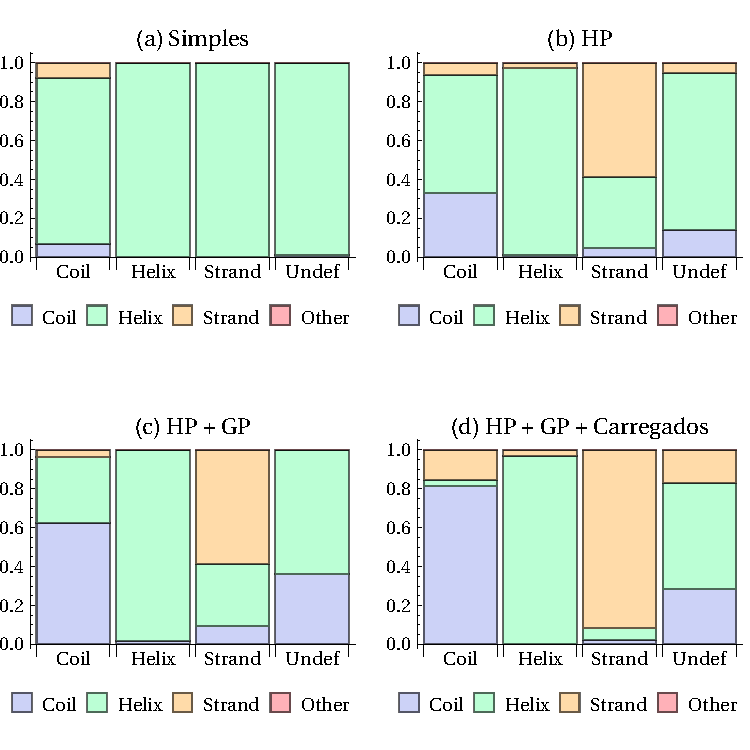
\includegraphics[width=.9\textwidth]{figures/chamel_errors_ca.pdf}
  \caption{Figura da sequencia e das estruturas das camaleonicas}
        \label{fig:ca_errors}
\end{figure}

\begin{figure}
  \centering
  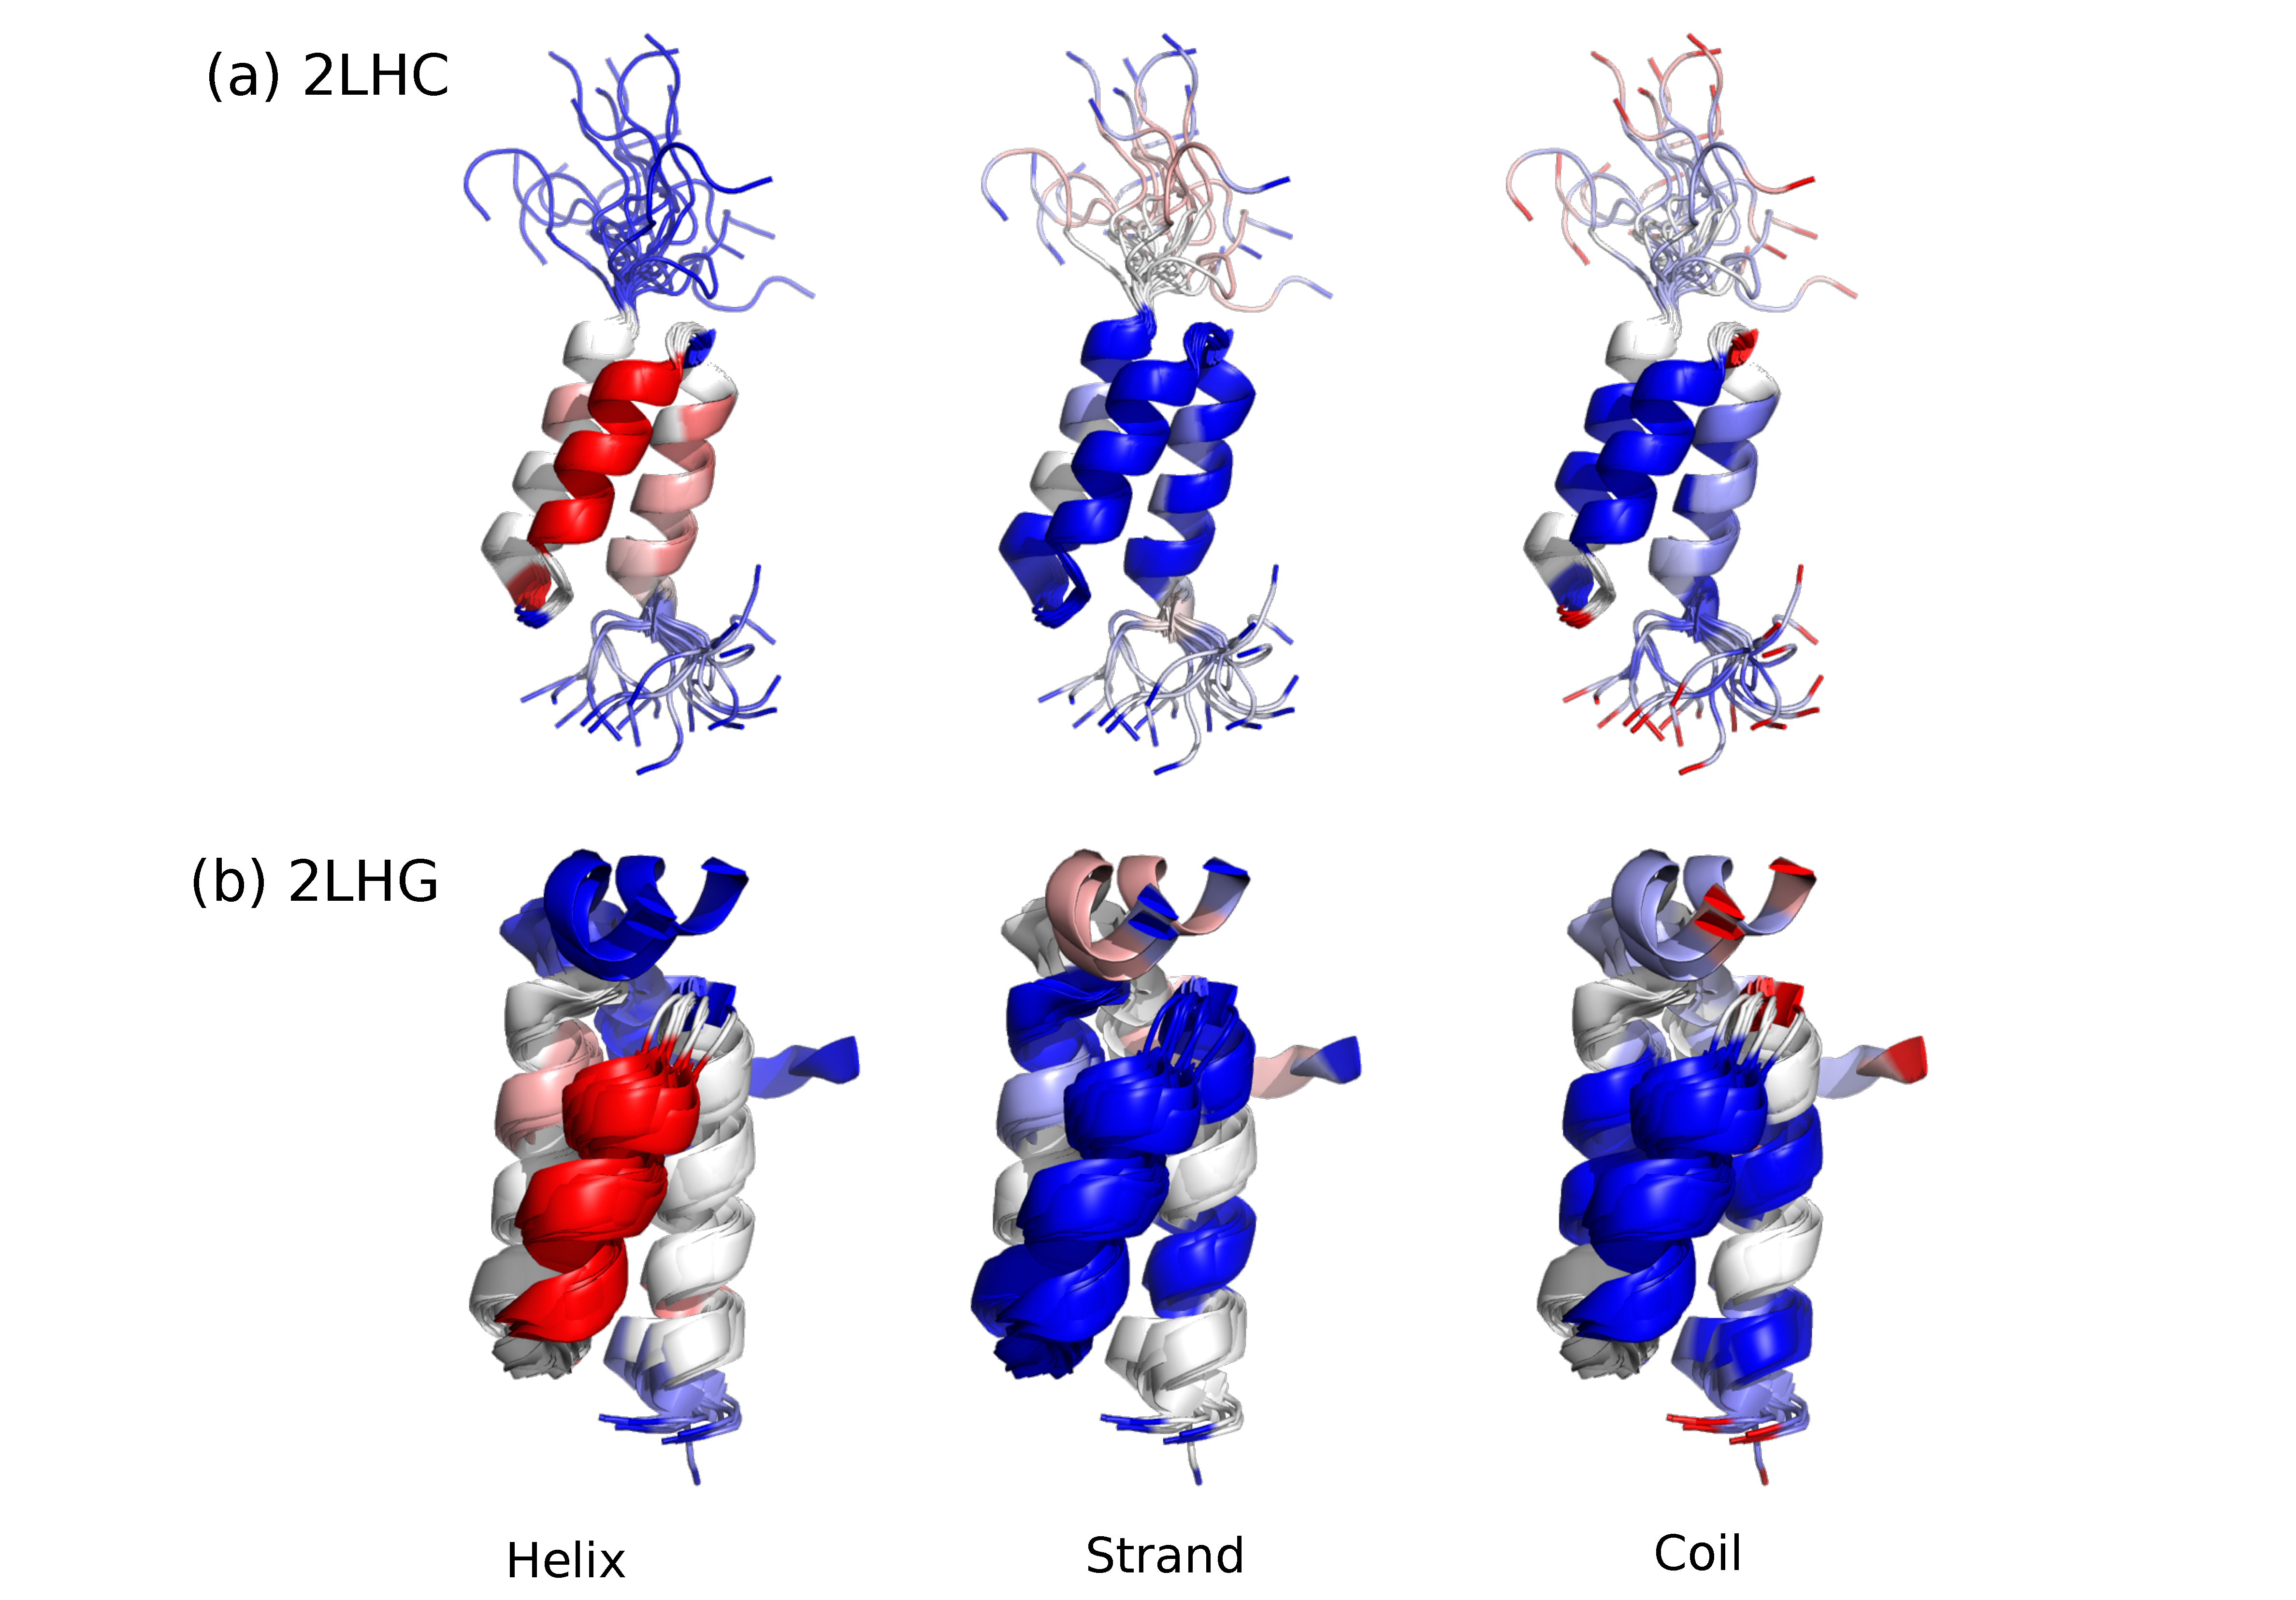
\includegraphics[width=1\textwidth]{figures/camel_2lhc_2lhg.pdf}
  \caption{Figura da sequencia e das estruturas das camaleonicas}
        \label{fig:camel_2lhc_2lhg}
\end{figure}

\begin{figure}
  \centering
  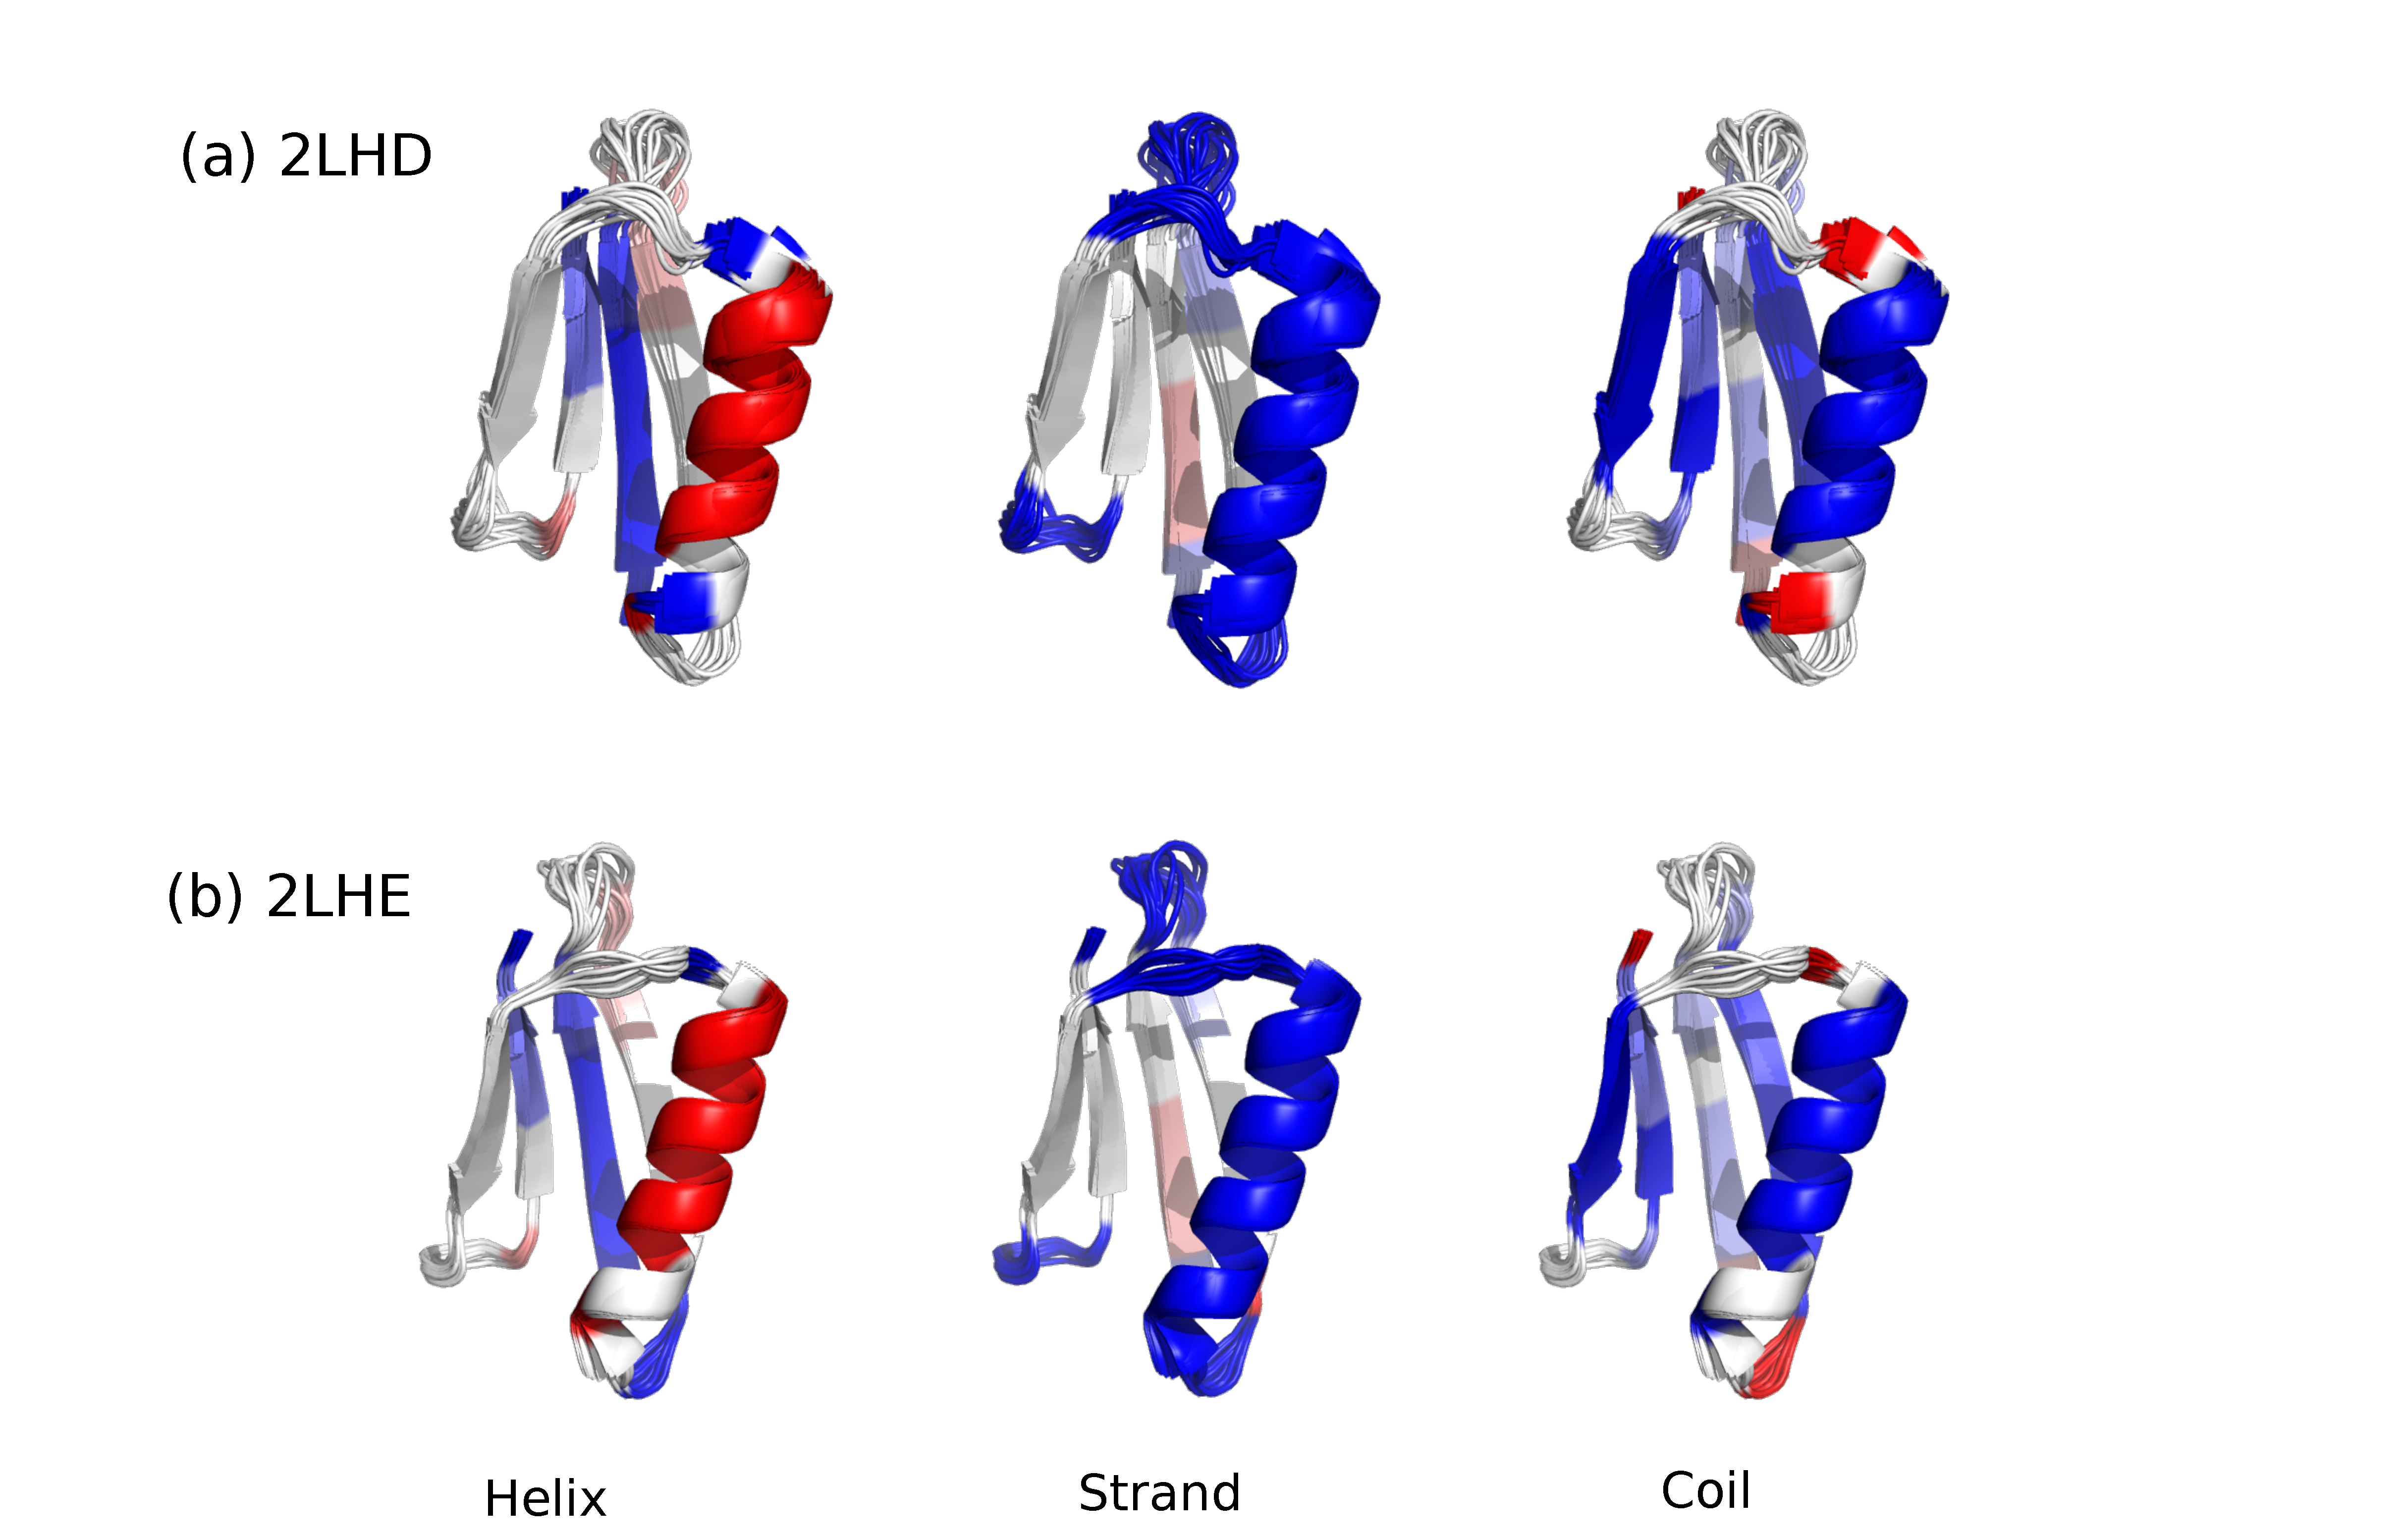
\includegraphics[width=1\textwidth]{figures/camel_2lhd_2lhe.pdf}
  \caption{Figura da sequencia e das estruturas das camaleonicas}
        \label{fig:camel_2lhd_2lhe}
\end{figure}


\section{EDA}

O aprendizado das regras realizado através de um algoritmo de EDA distribuído demonstrou-se eficiente dado a complexidade do problema. Utilizando sete nós (448 núcleos) no cluster multiusuário da FAPESP localizado no Centro Internacional de Pesquisa e Ensino do Hospital A. C. Camargo em  São Paulo foi possível evoluir o EDA por 1000 gerações com 10000 indivíduos em pouco menos de duas semanas.

Cada nó de trabalho apresentou um uso de memória de 75\% (48 GB), e manteve o processamento próximo a 100\% por núcleo (1.6 GHz). O mecanismo de comunicação por RPC entre o nó mestre e os nós de trabalho não sobrecarregou a rede (1Gbs). Isso nos permite concluir que o algoritmo é escalável clusters com maior número de nós e processadores de maior desempenho.

A opção por realizar o torneio entre soluções candidatas nos nós de trabalho, permite apenas a opção de realizar o torneio entre as k últimas soluções geradas no próprio nó. Consequentemente, as k-1 soluções perdedoras são descartadas, havendo portanto, a remoção das soluções perdedoras em cada torneio. 

Usualmente, o método de seleção por torneio utilizado em algoritmos genéticos não distribuídos acumula as solução candidatas até atingir o tamanho máximo populacional, quando então, é realizado o torneio. Isso permite que o torneio seja feito sem a eliminação dos perdedores, possibilitando que a seleção destes ocorram em outros combates.

Entretanto, no EDA distribuído, para aplicarmos um torneio sem eliminação dos perdedores seria necessário:

\begin{enumerate}
	\item o envio de todas as soluções candidatas para o nó mestre, o que resultaria em maior consumo de rede;
	\item o acúmulo de todas as soluções candidatas até atingir o tamanho máximo da população, gerando uma limitação da memória disponível;
	\item a espera até a realização do torneio para iniciar o cálculo das probabilidades, resultando no aumento do tempo ocioso nos nós de trabalho igual ao intervalo de tempo do envio da última solução até o cálculo das probabilidades.
\end{enumerate} 

A escolha em realizar o torneio nos nós de trabalho demonstrou ser escalável, manter a variabilidade das soluções candidatas ao longo da evolução e convergência (Figura \ref{fig:evo_eda}).

\begin{figure}
  \centering
  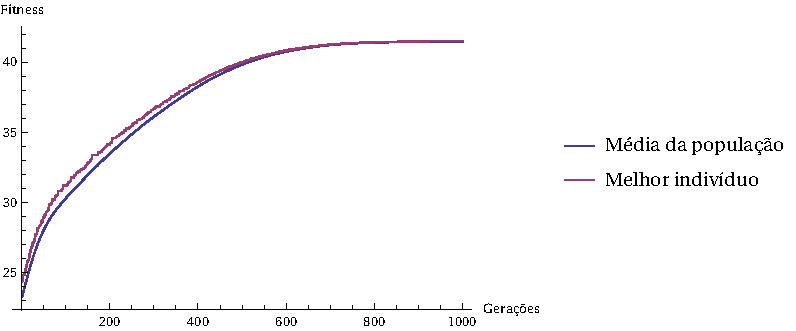
\includegraphics[width=1\textwidth]{figures/evo_Eda.pdf}
  \caption{EDA}
        \label{fig:evo_eda}
\end{figure}

\subsection{Deriva genética}

A evolução do EDA por 1000 gerações com torneio de dois (k=2) e população de 10000 indivíduos, demonstrou sinais de deriva genética a partir de 564 gerações. Tais sinais podem ser detectados observando-se as probabilidades dos 38 elementos de regra que não ocorrem no conjunto de proteínas. Esses elementos são do tipo [\#][\textit{x}][\#].

O elementos [\#][\textit{x}][\#], onde o \textit{x} correponde a qualquer estado exceto [\#], não apresentam probabilidade fixa, mas também, por estar ausente nas proteínas, não sofrem pressão seletiva. Logo, suas variações são aleatórias.

Na geração 564 um desses 38 elementos apresentou probabilidade zero ($p=0$), de transitar para um dos quatro estados possíveis, indicando a eliminação de um gene da população por deriva genética. Ao final das 1000 gerações 11 dos 38 elementos apresentavam probabilidade zero para uma das transições (Figura \ref{fig:deriva_genetica}).

\begin{figure}
  \centering
  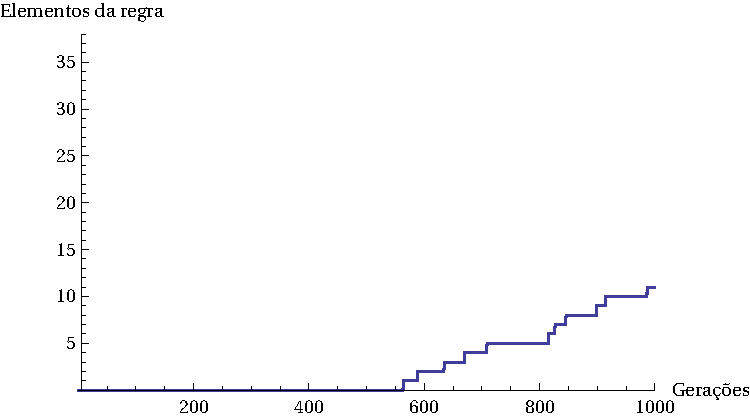
\includegraphics[width=1\textwidth]{figures/deriva_genetica.pdf}
  \caption{Deriva genetica}
        \label{fig:deriva_genetica}
\end{figure}

\subsection{Função de fitness}

A simplicidade da equação de fitness (referencia a equaçao) demonstrou problemas que acreditamos serem solucionáveis na continuação deste trabalho. Um desses problemas é ocasionado pelo desbalanceamento dos dados de treinamento (Figura \ref{fig:occ_ss}). 

\begin{figure}
  \centering
  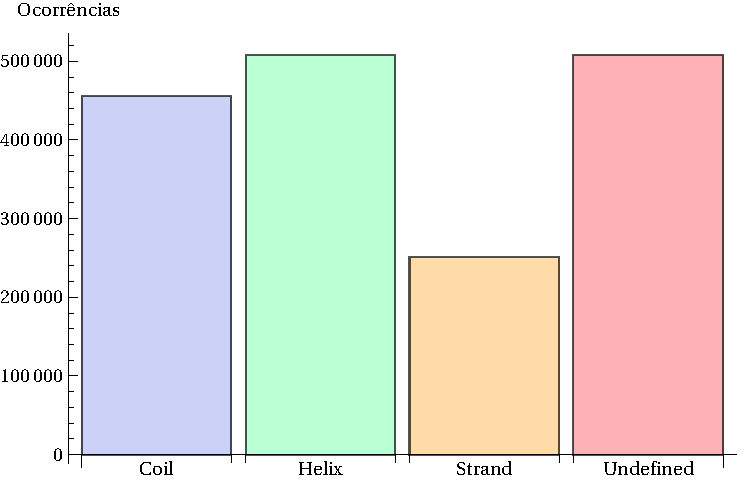
\includegraphics[width=0.9\textwidth]{figures/occ_ss.pdf}
  \caption{Desbalanceamento elementos de estrutura secundária no conjunto de dados}
        \label{fig:occ_ss}
\end{figure}

Os resultados obtidos indicam uma maior acurácia para os elementos de estrutura secundária mais frequentes no conjunto de treinamento. Esse é um problema recorrente no aprendizado com classes desbalanceadas e costuma ser tratado na função de fitness (Figura \ref{fig:q3}). 

\begin{figure}
  \centering
  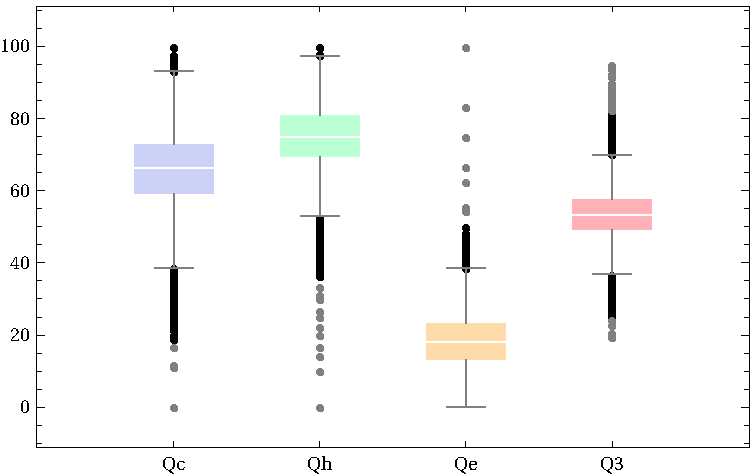
\includegraphics[width=0.9\textwidth]{figures/q3.pdf}
  \caption{q3}
        \label{fig:q3}
\end{figure}

% Avaliamos também se havia alguma relação aparente dos elementos preditos com os ângulos phi e psi do resíduos, o que poderia justificar parcilamente  erros nos elementos preditos. Entretanto, aparentemente não existe tal relação (figuras).



% Roc curve

%Outra modificação possível na função de fitness seria buscar a maximização da frequência dos estados durante a evolução do autômato.  

\subsection{Seleção}

As ocorrência de trincas no conjunto de proteínas apresentou grande variação (Figura \ref{fig:histograma_occ}). Para avaliar a influência do número de ocorrências das trincas na seleção do EDA nós procuramos por correlações entre fatores que poderiam influenciar na seleção.

\begin{figure}
  \centering
  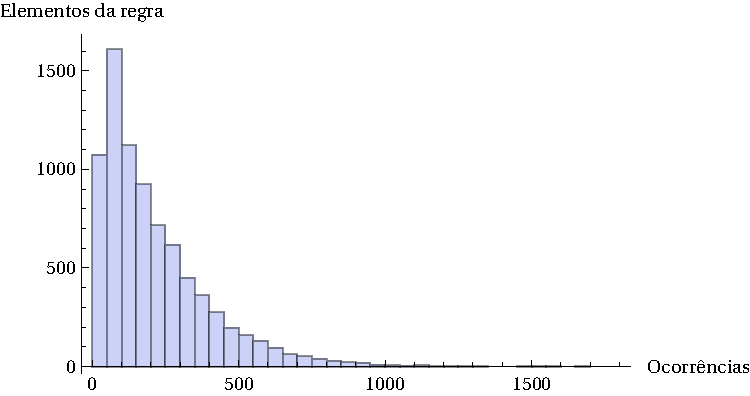
\includegraphics[width=1\textwidth]{figures/histograma_occ.pdf}
  \caption{Histograma de ocorrencia das trincas}
        \label{fig:histograma_occ}
\end{figure}

A figura \ref{fig:probG999_occXprob} representa a distribuição das probabilidades máximas e mínimas das dos elementos da regra em relação a frequência de ocorrência das trincas no conjunto. O gráfico e o valor de correlação (Spearman = 0.09) entre as probabilidades e a frequência de ocorrência das trincas,  indica não haver uma grande influência da frequência das trincas durante a seleção. Essa influência também não foi encontrada durante a evolução do EDA (Anexo).  

\begin{figure}
  \centering
  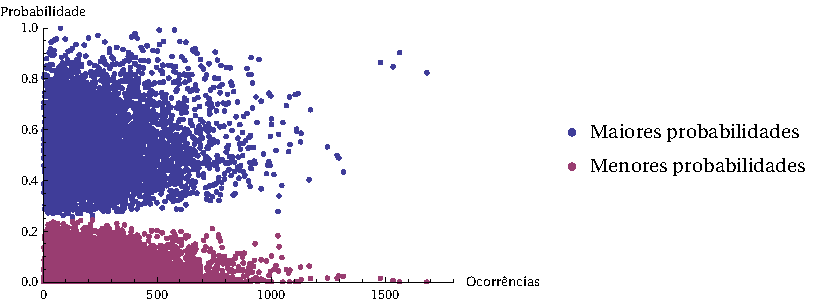
\includegraphics[width=1\textwidth]{figures/probG999_occXprob.pdf}
  \caption{Probabilidades máximas e mínimas pelo numero de corrência das trincas}
        \label{fig:probG999_occXprob}
\end{figure}


Outros fatores que poderiam influenciar a evolução do EDA seriam: \textit{(1)} a probabilidade da trinca ser observada em uma determinada estrutura secundária; \textit{(2)} o número de ocorrências da trinca em determinada estrutura secundária; \textit{(3)} a taxa de acertos por trincas para determinada estrutura secundária.     

As probabilidades de transição dos elementos da regra, não apresentam aparente relação com as proporções encontradas para cada estrutura secundária nas trincas (Figuras H E C).Assim como não apresentaram relação com a frequência de ocorrências de determinada estrutura para uma trinca e com a proporção de trincas corretamente classificadas por estrutura secundária. Essas duas últimas relações não eram mesmo esperadas (Anexo Figuras H E C e figuras H E C). Contudo, foi interessante observar que a primeira relação aparentemente não ocorria. 

\begin{figure}
  \centering
  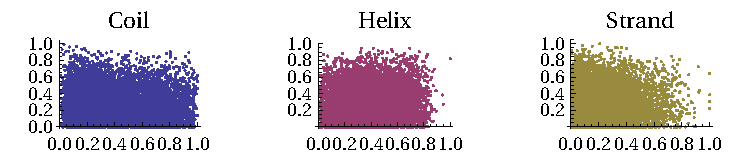
\includegraphics[width=1\textwidth]{figures/relacao_prob_propss.pdf}
  \caption{Relação proporção de ss nas trincas x probabilidade EDA}
        \label{fig:relacao_prob_propss}
\end{figure}

A ausência da primeira relação pode indicar que as probabilidades de transição dos demais elementos da regra e sua aplicação ao longo da evolução do CA estão propagando as probabilidades e sofrendo influência da vizinhança na busca de produzir estruturas secundárias mais próximas as reais. 

Entretanto, observamos uma relação entre a proporção de elementos de estruturas secundárias para um trinca e a proporção de acertos da trinca para a mesma estrutura secundária. Acreditamos que isso seja um indício que o aprendizado, ou otimização da regra, precisa ser melhorado para que elementos de estruturas secundárias menos comuns a determinadas trincas possam ser corretamente preditos (Figura \ref{fig:prop_acerto} e Tabela \ref{tab:corr_acertos}).  

\begin{figure}
  \centering
  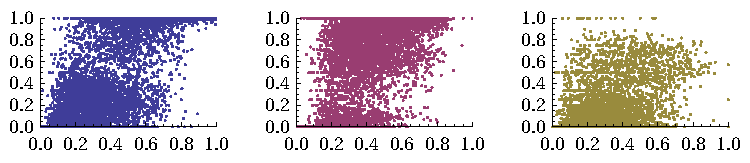
\includegraphics[width=1\textwidth]{figures/prop_acerto.pdf}
  \caption{Relação proporção de acertos x probabilidade EDA}
        \label{fig:prop_acerto}
\end{figure}

Há também uma relação menos influente entre o número de ocorrências de uma determinada estrutura secundária nas trincas e a proporção de acertos dessa trinca para a mesma estrutura secundária (Figura \ref{fig:occ_acerto} e Tabela \ref{tab:corr_acertos}).

\begin{figure}
  \centering
  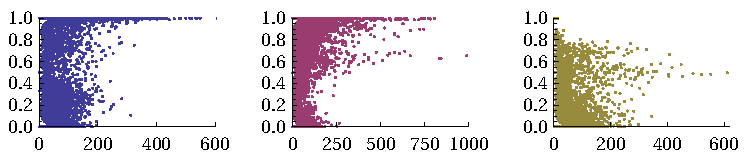
\includegraphics[width=1\textwidth]{figures/occ_acerto.pdf}
  \caption{Relação ocorrencias das ss por trincas x probabilidade EDA}
        \label{fig:occ_acerto}
\end{figure}

\begin{table}
    \myfloatalign
    \label{tab:corr_acertos}
  \begin{tabularx}{\textwidth}{Xlll} \toprule
    \tableheadline{Correlação}   & \tableheadline{coil}   & \tableheadline{hélices}  & \tableheadline{fitas} \\ 
    \midrule
     Proporção das trincas  & 0,75 & 0,60   & 0,60   \\
    Ocorrências das trincas  & 0,60 & 0,24   & 0,38  \\
    %autem vulputate ex & parola & romanic \\
    %usu mucius iisque & studio & sanctificatef \\
    \bottomrule
  \end{tabularx}
  \caption{Correlação (Spearman) entre a proporção de acertos na predição e: (1) proporção das trincas nas estruturas secundárias, (2) número de ocorrências das trincas nas estruturas secundárias}
\end{table}

Ambas as relações encontradas eram esperadas pois indicam uma tendência do método a privilegiar o aprendizado, ou otimizaração, de elementos capazes de influenciar com maior intensidade a função de fitness. Isso mostra a importância de manter um variabilidade alta na população e reduzir efeitos de deriva genética para que a otimização escape de mínimos locais e consiga aprender, também, as probabilidades para trincas menos frequentes nas proteínas e/ou com proporções pequenas para determinadas estruturas secundárias.






\section{proteina?}






A proteína Ga98 e seus mutantes, os quais sofrem alterações globais na estrutura secundária, são casos interessantes para o teste de novas metodologias de predição de estrutura secundária. Nas metodologias atuais, que comumente utilizam redes neurais, a predição é feita utilizando uma janela de resíduos, em geral com comprimentos de 9, 11 ou 13 resíduos, onde o resíduo central da janela é classificado pela rede neural. Como a predição nas demais janelas presentes na sequência polipeptídica não influencia na classificação da janela, o método apresenta a limitação de responder apenas localmente às variações dos dados de entrada.  

Por outro lado, os autômatos celulares, apesar de evoluirem de acordo com regras locais, tem a capacidade de propagar as variações locais e influenciar o surgimento ou alteração de padrões globais, distantes do ponto de origem da variação. 

Para avaliar a capacidade dos modelos propostos e da eficácia do método de otimização em encontrar regras capazes de reproduzir o padrão correspondente às estruturas secundárias, testamos a nossa metodologia nessas quatro proteínas.



\chapter{Aprendizado das regras gerais}




% \section{contagem de aa}
% CCW      2
% CMW      2
% WMC      2
% WPC      3
% WCW      3
% CHW      4
% MWC      4
% CCC      4
% CMC      4
% WCC      4
% CWW      4
% WWM      5
% MCW      5
% CWC      5
% MWM      6
% CCM      6
% MWH      6
% CWH      6
% FWC      6
% QCC      6
% QCW      6
% WWW      6
% WCH      7
% CMM      7
% YCW      7
% WCM      7
% CIW      7
% HWC      7
% CQW      7
% CYW      8
% ..     ...
% AAE   1000
% LKE   1001
% AEA   1011
% EAA   1021
% AGA   1029
% AGL   1032
% AAV   1034
% AEL   1046
% ELA   1051
% EEL   1066
% ALG   1076
% LGL   1080
% LAG   1082
% VAA   1105
% ALE   1111
% LEA   1111
% AVA   1118
% ELL   1129
% LAL   1131
% LLE   1166
% LAE   1172
% AAG   1246
% ALL   1289
% LLA   1296
% EAL   1316
% LAA   1478
% AAL   1534
% ALA   1563
% AAA   1682
% HHH   6143